% SIAM Article Template
\documentclass[review,hidelinks,onefignum,onetabnum]{siamart220329}

% Information that is shared between the article and the supplement
% (title and author information, macros, packages, etc.) goes into
% ex_shared.tex. If there is no supplement, this file can be included
% directly.

% SIAM Shared Information Template
% This is information that is shared between the main document and any
% supplement. If no supplement is required, then this information can
% be included directly in the main document.


% Packages and macros go here
\usepackage{lipsum}
\usepackage{amsfonts}
\usepackage{graphicx}
\usepackage{epstopdf}
\usepackage{algorithmic}
\ifpdf
  \DeclareGraphicsExtensions{.eps,.pdf,.png,.jpg}
\else
  \DeclareGraphicsExtensions{.eps}
\fi

% Add a serial/Oxford comma by default.
\newcommand{\creflastconjunction}{, and~}

% Used for creating new theorem and remark environments
\newsiamremark{remark}{Remark}
\newsiamremark{hypothesis}{Hypothesis}
\crefname{hypothesis}{Hypothesis}{Hypotheses}
\newsiamthm{claim}{Claim}

% Sets running headers as well as PDF title and authors
\headers{A second order numerical methods for Reisz-Fractional Elliptic Equation on graded mesh }{Jianxing Han and Minghua Chen}

% Title. If the supplement option is on, then "Supplementary Material"
% is automatically inserted before the title.
\title{second-order error analysis for Fractional Laplacian via Riesz Derivatives on graded meshes\thanks{Submitted to the editors DATE.
}}

% Authors: full names plus addresses.
\author{Jianxing Han\thanks{School of Mathematics and Statistics, Lanzhou University, Lanzhou 730000, PR China
  (\email{hanjx2023@mail.lzu.edu.cn}).}
  \and Minghua Chen\thanks{School of Mathematics and Statistics, Lanzhou University, Lanzhou 730000, PR China 
  (\email{chen@mail.lzu.edu.cn}).}
}

\usepackage{amsopn}
\DeclareMathOperator{\diag}{diag}


%%% Local Variables: 
%%% mode:latex
%%% TeX-master: "ex_article"
%%% End: 


% Optional PDF information
\ifpdf
\hypersetup{
  pdftitle={An Example Article},
  pdfauthor={D. Doe, P. T. Frank, and J. E. Smith}
}
\fi

% The next statement enables references to information in the
% supplement. See the xr-hyperref package for details.

\externaldocument[][nocite]{ex_supplement}

% FundRef data to be entered by SIAM
%<funding-group specific-use="FundRef">
%<award-group>
%<funding-source>
%<named-content content-type="funder-name"> 
%</named-content> 
%<named-content content-type="funder-identifier"> 
%</named-content>
%</funding-source>
%<award-id> </award-id>
%</award-group>
%</funding-group>

\begin{document}

\maketitle

% REQUIRED
\begin{abstract}
  This is an example SIAM \LaTeX\ article. This can be used as a
  template for new articles.  Abstracts must be able to stand alone
  and so cannot contain citations to the paper's references,
  equations, etc.  An abstract must consist of a single paragraph and
  be concise. Because of online formatting, abstracts must appear as
  plain as possible. Any equations should be inline.
\end{abstract}

% REQUIRED
\begin{keywords}
  example, \LaTeX
\end{keywords}

% REQUIRED
\begin{MSCcodes}
  68Q25, 68R10, 68U05
\end{MSCcodes}

\section{Introduction}
The introduction introduces the context and summarizes the
manuscript. It is importantly to clearly state the contributions of
this piece of work.

\textcolor{blue}{
  For \(\Omega=(0,2T)\), \(1<\alpha<2\), suppose \(f\in C^2(\Omega)\)
  \begin{equation} \label{eq:equation}
    \begin{cases}
      (-\Delta)^{\frac{\alpha}{2}} u(x) = f(x), & x \in \Omega                      \\
      u(x) = 0,                                 & x \in \mathbb{R} \setminus \Omega
    \end{cases}
  \end{equation}
  where
  \begin{equation} \label{def:operator}
    (-\Delta)^{\frac{\alpha}{2}} u(x) = -\frac{\partial^\alpha u}{\partial |x|^\alpha}
    = -\kappa_\alpha \frac{d^2}{dx^2} \int_\Omega \frac{|x-y|^{1-\alpha}}{\Gamma(2-\alpha)}u(y) dy
  \end{equation}
  \begin{equation} \label{def:kappa}
    \kappa_\alpha = -\frac{1}{2\cos(\alpha\pi/2)} > 0
  \end{equation}
}

\textcolor{orange}{
  \begin{theorem} \label{thm:regularity}
    Let $u$ be a solution of \eqref{eq:equation} on $\Omega$. Then, for any $x\in\Omega$ and \(l=0, 1, 2, 3, 4\)
    \begin{equation}
      |u^{(l)}(x)| \le C [x(2T-x)]^{\alpha/2-l}
    \end{equation}
  \end{theorem}
}


% The outline is not required, but we show an example here.
The paper is organized as follows. Our main results are in
\cref{sec:main},  experimental
results are in \cref{sec:experiments}, and the conclusions follow in
\cref{sec:conclusions}.


\section{Numeric Format}
\label{sec:numformat}


\textcolor{blue}{
  \begin{equation} \label{def:xj}
    x_i = \begin{cases}
      T \left(\frac{i}{N}\right)^r   ,      & 0 \le i \le N  \\
      2T - T \left(\frac{2N-i}{N}\right)^r, & N \le i \le 2N
    \end{cases}
  \end{equation}
  where $r\ge 1$ .
  And let
  \begin{equation} \label{def:hj}
    h_j = x_{j} - x_{j-1}, \quad 1\le j \le 2N
  \end{equation}
}

\textcolor{blue}{
Let $\{\phi_j(x)\}_{j=1}^{2N-1}$ be standard hat functions, which are basis of the piecewise linear function space.
\begin{equation}
  \phi_j(x) = \begin{cases}
    \frac{1}{h_j} (x-x_{j-1}),      & x_{j-1} \le x \le x_{j} \\
    \frac{1}{h_{j+1}} (x_{j+1}-x) , & x_{j} \le x \le x_{j+1} \\
    0,                              & \text{otherwise}
  \end{cases}
\end{equation}
And then, we can approximate $u(x)$ with
\begin{equation}
  u_h(x) := \sum_{j=1}^{2N-1} u(x_j) \phi_j(x)
\end{equation}
}

\textcolor{blue}{
  For convience, we denote
  \begin{equation} \label{def:Ih}
    I_h^{2-\alpha}(x) := \frac{1}{\Gamma(2-\alpha)}\int_{\Omega} |x-y|^{1-\alpha} u_h(y) dy
  \end{equation}
  And now, we can approximate the operator \eqref{def:operator} at $x_i$ with
  \begin{equation} \label{def:Dhalpha}
    \begin{aligned}
      D_h^{\alpha} u_h(x_i) & := D_h^2 I_h^{2-\alpha}(x_i) \\
                            & =\frac{2}{h_{i} + h_{i+1}}
      \left( \frac{1}{h_{i}} I_h^{2-\alpha}(x_{i-1}) - \left( \frac{1}{h_{i}} + \frac{1}{h_{i+1}} \right) I_h^{2-\alpha}(x_{i}) + \frac{1}{h_{i+1}} I_h^{2-\alpha}(x_{i+1}) \right)
    \end{aligned}
  \end{equation}
  Finally, we approximate the equation \eqref{eq:equation} with
  \begin{equation} \label{def:discrete_equation}
    -\kappa_\alpha D_h^{\alpha} u_h(x_i) = f(x_i), \quad 1\le i \le 2N-1
  \end{equation}
}


\textcolor{blue}{
  The discrete equation \eqref{def:discrete_equation} can be written in matrix form
  \begin{equation} \label{eq:equation_matrix}
    AU = F
  \end{equation}
  where $U$ is unknown, $F=(f(x_1), \cdots, f(x_{2N-1}))$.
  The matrix $A$ is constructed as follows:
  Since
  \begin{equation}
    \begin{aligned} \label{eq:Ih}
      I_h^{2-\alpha}(x_i) & = \frac{1}{\Gamma(2-\alpha)} \int_{\Omega} |x_i-y|^{1-\alpha} u_h(y) dy                                                                     \\
                          & = \sum_{j=1}^{2N-1} \frac{1}{\Gamma(2-\alpha)} \int_{\Omega} |x_i-y|^{1-\alpha} u(x_j) \phi_j(y) dy                                         \\
                          & = \sum_{j=1}^{2N-1} u(x_j)  \frac{1}{\Gamma(2-\alpha)} \int_{x_{j-1}}^{x_{j+1}} |x_i-y|^{1-\alpha} \phi_j(y) dy                             \\
                          & = \sum_{j=1}^{2N-1} \frac{u(x_j)}{\Gamma(4-\alpha)}
      \left( \frac{|x_{i}-x_{j-1}|^{3-\alpha}}{h_{j}} -\frac{h_{j} + h_{j+1}}{h_{j}h_{j+1}}|x_i-x_{j}|^{3-\alpha} +  \frac{|x_{i}-x_{j+1}|^{3-\alpha}}{h_{j+1}} \right) \\
                          & =: \sum_{j=1}^{2N-1} \tilde{a}_{ij} \; u(x_j), \quad 0 \le i \le 2N
    \end{aligned}
  \end{equation}
  Then, substitute in \eqref{def:Dhalpha}, we have
  \begin{equation}
    -\kappa_\alpha  D_h^{\alpha} u_h(x_i) = \sum_{j=1}^{2N-1} a_{ij} \; u(x_j)
  \end{equation}
  where
  \begin{equation} \label{mat:aij}
    a_{ij} = -\kappa_\alpha \frac{2}{h_{i} + h_{i+1}}
    \left( \frac{1}{h_{i}} \tilde{a}_{i-1,j} - \left( \frac{1}{h_{i}} + \frac{1}{h_{i+1}} \right) \tilde{a}_{i,j} +  \frac{1}{h_{i+1}} \tilde{a}_{i+1, j} \right)
  \end{equation}
}


\section{Main results}
\label{sec:main}


Here we state our main results; the proof is
deferred to \cref{sec:proof-truncation-error} and \cref{sec:proof-convergence}.

\textcolor{blue}{
  Let's denote \(h=\frac{1}{N}\), we have
  \begin{theorem}[Truncation Error] \label{thm:truncation-error}
    If $f \in C^2(\Omega)$ and $\alpha\in(1,2)$, and $u(x)$ is a solution of the equation \eqref{eq:equation}, then there exists a constant
    $C=C(T,\alpha, r, \|f\|_{C^2(\Omega)})$, such that
    the truncation error of the discrete format satisfies
    \begin{equation} \label{eq:truncation-error}
      \begin{aligned}
        | -\kappa_\alpha D_h^{\alpha} u_h(x_i) - f(x_i) |
        \le & C ( h^{r\alpha/2+r}(x_i^{-1-\alpha}+(2T-x_i)^{-1-\alpha}) \\
            & + h^2(x_i^{-\alpha/2-2/r} + (2T-x_i)^{-\alpha/2-2/r})     \\
            & + h^2
        \begin{cases}
          |T-x_{i-1}|^{1-\alpha}, \quad 1\le i\le N \\
          |T-x_{i+1}|^{1-\alpha} , \quad N<i\le 2N-1
        \end{cases} )
      \end{aligned}
    \end{equation}
  \end{theorem}
}


\textcolor{blue}{
  \begin{theorem}[Convergence]\label{thm:convergence}
    The discrete equation \eqref{def:discrete_equation} has sulotion $U$,
    and there exists a positive constant $C=C(T,\alpha, r, \|f\|_{C^2(\Omega)})$
    such that the error between the numerial solution $U$ with the exact solution $u(x_i)$ satisfies
    \begin{equation} \label{eq:error}
      \max_{1\le i \le 2N-1} |U_i - x(x_i)| \le C h^{\min\{\frac{r\alpha}{2}, 2\}}
    \end{equation}
    That means the numerial method has convergence order ${\min\{\frac{r\alpha}{2}, 2\}}$.
  \end{theorem}
}



\section{Proof of \cref{thm:truncation-error}}
\label{sec:proof-truncation-error}

\textcolor{blue}{
  For convience, let's denote
  \begin{equation}
    I^{2-\alpha}(x) = \frac{1}{\Gamma(2-\alpha)} \int_{\Omega} |x-y|^{1-\alpha} u(y) dy
  \end{equation}
  Then, the truncation error of the discrete format can be written as
  \begin{equation}
    \begin{aligned}
      - \kappa_\alpha D_h^{\alpha} u_h(x_i) - f(x_i)
       & = -\kappa_\alpha (D_h^2 I_h^{2-\alpha}(x_i) - \frac{d^2}{dx^2} I^{2-\alpha}(x_i))                                           \\
       & = -\kappa_\alpha D_h^2 (I_h^{2-\alpha}(x_i)-I^{2-\alpha}(x_i)) - \kappa_\alpha (D_h^2 - \frac{d^2}{dx^2}) I^{2-\alpha}(x_i) \\
    \end{aligned}
  \end{equation}
}


\textcolor{orange}{
  \begin{theorem} \label{lmm:trunerror2}
    There exits a constant $C=C(T, r, \|f\|_{C^2(\Omega)})$ such that
    \begin{equation}
      -\kappa_\alpha (D_h^2 - \frac{d^2}{dx^2}) I^{2-\alpha} (x_i) \le C h^2 (x_i^{1-2/r} + (2T-x_i)^{1-2/r})
    \end{equation}
  \end{theorem}
  \begin{proof}
    Since \(f\in C^2(\Omega)\) and
    \begin{equation}
      \frac{d^2}{dx^2} ( - \kappa_\alpha I^{2-\alpha}(x)) = f(x),  \quad x \in \Omega,
    \end{equation}
    we have \(I^{2-\alpha} \in C^4(\Omega)\).
    Therefore, using equation \cref{eq:D2simd4} of \cref{lmm:D2simd2}, for \(1\le i\le 2N-1\), we have
    \begin{equation}
      \begin{aligned}
        -\kappa_\alpha (D_h^2 - \frac{d^2}{dx^2}) I^{2-\alpha} (x_i)
         & = \frac{h_{i+1}-h_{i}}{3} f'(x_i) + \frac{1}{4!} \frac{2}{h_i + h_{i+1}}(h_i^3 f''(\eta_1) + h_{i+1}^3 f''(\eta_2))   \\
      \end{aligned}
    \end{equation}
    where \(\eta_1 \in [x_{i-1}, x_{i}], \eta_2 \in [x_{i}, x_{i+1}]\).
    By \cref{lmm:hi1-hi}, we have
    1.
    \begin{equation}
      \left| \frac{h_{i+1}-h_{i}}{3} f'(x_i) \right| \le \frac{\|f\|_{C^1(\Omega)}}{3} 2^{|r-2|}r(r-1)T^{2/r} h^2 (x_i^{1-2/r} + (2T-x_i)^{1-2/r})
    \end{equation}
    2.
    \begin{equation}
      \begin{aligned}
        \frac{1}{4!} \frac{2}{h_i + h_{i+1}} & (h_i^3 f''(\eta_1) + h_{i+1}^3 f''(\eta_2))  \\
        &\le \frac{\|f\|_{C^2(\Omega)}}{12} (h_i^2-h_{i}h_{i+1}+h_{i+1}^2)
      \end{aligned}
    \end{equation}
  \end{proof}
}



\section{Proof of \cref{thm:convergence}}
\label{sec:proof-convergence}

\textcolor{orange}{
  aaaaaaaaaa
}


\section{Experimental results}
\label{sec:experiments}


\Cref{fig:testfig} shows some example results. Additional results are
available in the supplement in \cref{tab:foo}.

\begin{figure}[htbp]
  \centering
  \label{fig:a}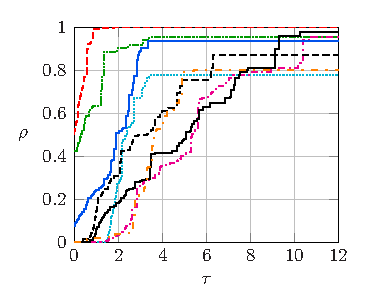
\includegraphics{lexample_fig1}
  \caption{Example figure using external image files.}
  \label{fig:testfig}
\end{figure}

\Cref{tab:foo} shows additional
supporting evidence.

\begin{table}[htbp]
  \footnotesize
  \caption{Example table.}\label{tab:foo}
  \begin{center}
    \begin{tabular}{|c|c|c|} \hline
      Species & \bf Mean & \bf Std.~Dev. \\ \hline
      1       & 3.4      & 1.2           \\
      2       & 5.4      & 0.6           \\
      3       & 7.4      & 2.4           \\
      4       & 9.4      & 1.8           \\ \hline
    \end{tabular}
  \end{center}
\end{table}

\lipsum[51]

\section{Discussion of \texorpdfstring{{\boldmath$Z=X \cup Y$}}{Z = X union Y}}

\lipsum[76]

\section{Conclusions}
\label{sec:conclusions}

Some conclusions here.


\appendix

\section{Approximate of difference quotients}

\textcolor{blue}{
  \begin{lemma} \label{lmm:D2simd2}
    If \(g(x)\) is twice differentable continous function on open set $\Omega$,
    there exists \(\xi \in [x_{i-1}, x_{i+1}]\) such that
    \begin{equation} \label{eq:D2simd2}
      \begin{aligned}
        \frac{2}{h_i + h_{i+1}} & \left( \frac{1}{h_{i+1}} g(x_{i+1}) - (\frac{1}{h_{i}}+\frac{1}{h_{i+1}})g(x_{i}) + \frac{1}{h_{i}} g(x_{i-1}) \right) \\
        % &= \frac{h_i}{h_i + h_{i+1}} g''(\xi_1) + \frac{h_{i+1}}{h_i + h_{i+1}} g''(\xi_2)  \\
                                & = g''(\xi), \quad \xi \in [x_{i-1}, x_{i+1}]
      \end{aligned}
    \end{equation}
    And if \(g(x) \in C^4(\Omega)\), then
    \begin{equation} \label{eq:D2simd4}
      \begin{aligned}
        \frac{2}{h_i + h_{i+1}} & \left( \frac{1}{h_{i+1}} g(x_{i+1}) - (\frac{1}{h_{i}}+\frac{1}{h_{i+1}})g(x_{i}) + \frac{1}{h_{i}} g(x_{i-1}) \right)                   \\
                                & = g''(x_{i}) + \frac{h_{i+1}-h_{i}}{3} g'''(x_{i}) + \frac{1}{4!} \frac{2}{h_i + h_{i+1}}(h_i^3 g''''(\eta_1) + h_{i+1}^3 g''''(\eta_2))
      \end{aligned}
    \end{equation}
    where \(\eta_1 \in [x_{i-1}, x_{i}], \eta_2 \in [x_{i}, x_{i+1}]\).
  \end{lemma}
  \begin{proof}
    \begin{gather*}
      g(x_{i-1}) = g(x_{i}) - (x_{i}-x_{i-1}) g'(x_{i}) + \frac{(x_{i}-x_{i-1})^2}{2} g''(\xi_1), \quad \xi_1 \in [x_{i-1}, x_{i}]        \\
      g(x_{i+1}) = g(x_{i}) + (x_{i+1}-x_{i}) g'(x_{i}) + \frac{(x_{i+1}-x_{i})^2}{2} g''(\xi_2), \quad \xi_2 \in [x_{i}, x_{i+1}]
    \end{gather*}
    Subsitute them in the left side of \eqref{eq:D2simd2}, we have
    \begin{equation*}
      \begin{aligned}
        \frac{2}{h_i + h_{i+1}} & \left( \frac{1}{h_{i+1}} g(x_{i+1}) - (\frac{1}{h_{i}}+\frac{1}{h_{i+1}})g(x_{i}) + \frac{1}{h_{i}} g(x_{i-1}) \right) \\
                                & = \frac{h_i}{h_i + h_{i+1}} g''(\xi_1) + \frac{h_{i+1}}{h_i + h_{i+1}} g''(\xi_2)
      \end{aligned}
    \end{equation*}
    Now, using intermediate value theorem , there exists \(\xi \in [\xi_1, \xi_2]\) such that
    \begin{equation*}
      \frac{h_i}{h_i + h_{i+1}} g''(\xi_1) + \frac{h_{i+1}}{h_i + h_{i+1}} g''(\xi_2) = g''(\xi)
    \end{equation*}
    And for the second equation, similarly
    \begin{gather*}
      g(x_{i-1}) = g(x_{i}) - h_{i} g'(x_{i}) + \frac{h_{i}^2}{2} g''(x_{i}) - \frac{h_{i}^3}{3!} g'''(x_{i}) +  \frac{h_{i}^4}{4!} g''''(\eta_1)         \\
      g(x_{i+1}) = g(x_{i}) + h_{i+1} g'(x_{i}) + \frac{h_{i+1}^2}{2} g''(x_{i}) + \frac{h_{i+1}^3}{3!} g'''(x_{i}) + \frac{h_{i+1}^4}{4!} g''''(\eta_2)
    \end{gather*}
    where \(\eta_1 \in [x_{i-1}, x_{i}], \eta_2 \in [x_{i}, x_{i+1}]\).
    Subsitute them to the left side of \eqref{eq:D2simd4}, we can get the result.
  \end{proof}
}

\textcolor{blue}{
  \begin{lemma} \label{lmm:Dyj}
    If \(y\in [x_{j-1}, x_j]\), denote \(y = \theta x_{j-1} + (1-\theta) x_j, \theta\in [0,1]\),
    % then for \(2\le j \le 2N-1\)
    \begin{equation}
      \begin{aligned}
        u(y_j^\theta) - u_h(y_j^\theta) & = -\frac{\theta (1-\theta)}{2} h_j^2 u''(\xi), \quad \xi \in [x_{j-1}, x_j]
      \end{aligned}
    \end{equation}
    \begin{equation}
      \begin{aligned}
        u(y_j^\theta) - u_h(y_j^\theta) = & -\frac{\theta (1-\theta)}{2} h_j^2 u''(y_j^\theta)
        + \frac{\theta (1-\theta)}{3!} h_j^3 (\theta^2 u'''(\eta_1) - (1-\theta)^2 u'''(\eta_2))
      \end{aligned}
    \end{equation}
    where \(\eta_1 \in [x_{j-1}, y_j^\theta], \eta_2 \in [y_j^\theta, x_j]\).
  \end{lemma}
  \begin{proof}
    By Taylor expansion, we have
    \begin{gather*}
      u(x_{j-1}) = u(y_j^\theta) - \theta h_{j} u'(y_j^\theta) + \frac{\theta^2 h_{j}^2}{2!} u''(\xi_1), \quad \xi_1 \in [x_{j-1}, y_j^\theta] \\
      u(x_{j}) = u(y_j^\theta) + (1-\theta) h_{j} u'(y_j^\theta) + \frac{(1-\theta)^2 h_{j}^2}{2!} u''(\xi_2) , \quad \xi_2 \in [y_j^\theta, x_j]
    \end{gather*}
    Thus
    \begin{equation*}
      \begin{aligned}
        u(y_j^\theta) - u_h(y_j^\theta) & = u(y_j^\theta) - (1-\theta)u(x_{j-1}) - \theta u(x_{j})                          \\
                                        & = -\frac{\theta (1-\theta)}{2} h_j^2 (\theta u''(\xi_1) + (1-\theta) u''(\xi_2) ) \\
                                        & = -\frac{\theta (1-\theta)}{2} h_j^2 u''(\xi), \quad \xi \in [\xi_1, \xi_2]
      \end{aligned}
    \end{equation*}
    The second equation is similar,
    \begin{gather*}
      u(x_{j-1}) = u(y_j^\theta) - \theta h_{j} u'(y_j^\theta) + \frac{\theta^2 h_{j}^2}{2!} u''(y_j^\theta) - \frac{\theta^3 h_{j}^3}{3!} u'''(\eta_1)  \\
      u(x_{j}) = u(y_j^\theta) + (1-\theta) h_{j} u'(y_j^\theta) + \frac{(1-\theta)^2 h_{j}^2}{2!} u''(\xi_2) + \frac{(1-\theta)^3 h_{j}^3}{3!} u'''(\eta_2)
    \end{gather*}
    where \(\eta_1 \in [x_{j-1}, y_j^\theta], \eta_2 \in [y_j^\theta, x_j]\).
    Thus
    \begin{equation*}
      \begin{aligned}
        u(y_j^\theta) - u_h(y_j^\theta) & = u(y_j^\theta) - (1-\theta)u(x_{j-1}) - \theta u(x_{j})                                                                                      \\
                                        & = -\frac{\theta (1-\theta)}{2} h_j^2 u''(y_j^\theta) + \frac{\theta (1-\theta)}{3!} h_j^3 (\theta^2 u'''(\eta_1) - (1-\theta)^2 u'''(\eta_2))
      \end{aligned}
    \end{equation*}
  \end{proof}
}



\section{Inequality}

\textcolor{blue}{
  \begin{lemma}
    \begin{equation}
      h_i \le r T^{1/r} h \begin{cases}
        x_i^{1-1/r},          & 1\le i \le N   \\
        (2T-x_{i-1})^{1-1/r}, & N < i \le 2N-1
      \end{cases}
    \end{equation}
  \end{lemma}
  \begin{proof}
    For \(1\le i \le N\),
    \begin{displaymath}
      \begin{aligned}
        h_i & = T \left( \left(\frac{i}{N}\right)^r - \left(\frac{i-1}{N}\right)^r \right)  \\
            & \le rT \frac{1}{N} \left(\frac{i}{N}\right)^{r-1} = r T^{1/r} h x_{i}^{1-1/r} \\
      \end{aligned}
    \end{displaymath}
    For \(N < i \le 2N-1\),
    \begin{displaymath}
      \begin{aligned}
        h_i & = T\left( \left(\frac{2N-i}{N}\right)^r - \left(\frac{2N-i+1}{N}\right)^r \right)         \\
            & \le rT \frac{1}{N} \left(\frac{2N-i+1}{N}\right)^{r-1} = r T^{1/r} h (2T-x_{i-1})^{1-1/r} \\
      \end{aligned}
    \end{displaymath}
  \end{proof}
}


\textcolor{blue}{
  \begin{lemma} \label{lmm:hi1-hi}
    There is a constant \(C=2^{|r-2|}r(r-1)T^{2/r}\) such that for all \(i\in\{1,2,\cdots,2N-1\}\)
    \begin{equation}
      |h_{i+1} - h_{i}| \le C h^2 (x_i^{1-2/r} + (2T-x_i)^{1-2/r})
    \end{equation}
  \end{lemma}
  \begin{proof}
    \begin{equation*}
      \begin{aligned}
        h_{i+1} - h_{i} =
        \begin{cases}
          T \left( \left(\frac{i+1}{N}\right)^r - 2\left(\frac{i}{N}\right)^r + \left(\frac{i-1}{N}\right)^r  \right) ,           & 1\le i\le N-1    \\
          0,                                                                                                                      & i=N              \\
          -T \left( \left(\frac{2N-i-1}{N}\right)^r - 2\left(\frac{2N-i}{N}\right)^r + \left(\frac{2N-i+1}{N}\right)^r  \right) , & N+1\le i\le 2N-1 \\
        \end{cases}
      \end{aligned}
    \end{equation*}
    % if \(r=2\), 
    % \begin{equation*}
    %   h_{i+1}-h_{i} = 2T N^{-2}, \quad 1-2/r=0
    % \end{equation*}
    For \(i=1\),
    \begin{equation*}
      \begin{aligned}
        h_2-h_1 & = T(2^{r}-2)\left(\frac{1}{N}\right)^r = (2^{r}-2)T^{2/r} h^2 x_1^{1-2/r}
      \end{aligned}
    \end{equation*}
    For \(2\le i\le N-1\),
    \begin{equation*}
      \begin{aligned}
        h_{i+1} - h_{i} & =  r(r-1) T \; N^{-2} \eta^{r-2}, \quad \eta \in [\frac{i-1}{N}, \frac{i+1}{N}]
      \end{aligned}
    \end{equation*}
    If \(r\in[1, 2)\),
    \begin{equation*}
      \begin{aligned}
        h_{i+1} - h_{i} & \le  r(r-1) T \; N^{-2} \eta^{r-2}
        \le r(r-1) T \; h^2 \left( \frac{i-1}{N} \right)^{r-2}                         \\
                        & \le r(r-1) T \; h^2 2^{2-r} \left( \frac{i}{N} \right)^{r-2} \\
                        & = 2^{2-r} r(r-1) T^{2/r} h^2 x_i^{1-2/r}
      \end{aligned}
    \end{equation*}
    else if \(r>2\),
    \begin{equation*}
      \begin{aligned}
        h_{i+1} - h_{i} & \le  r(r-1) T \; N^{-2} \eta^{r-2}
        \le r(r-1) T \; h^2 \left( \frac{i+1}{N} \right)^{r-2}                         \\
                        & \le r(r-1) T \; h^2 2^{r-2} \left( \frac{i}{N} \right)^{r-2} \\
                        & = 2^{r-2} r(r-1) T^{2/r} h^2 x_i^{1-2/r}
      \end{aligned}
    \end{equation*}
    Since
    \begin{equation*}
      2^r-2 \le 2^{|r-2|}r(r-1), \quad r\ge 1
    \end{equation*}
    we have
    \begin{equation*}
      h_{i+1} - h_{i} \le 2^{|r-2|}r(r-1)T^{2/r} h^2 x_i^{1-2/r},  \quad 1\le i\le N-1
    \end{equation*}
    For \(i=N\), \( h_{N+1}-h_{N} = 0\).
    For \(N<i\le 2N-1\), it's central symmetric to the first half of the proof, which is
    % \begin{equation*}
    %   \begin{aligned}
    %     h_{2N-1} - h_{2N} & =
    %       T(2^{r}-2)\left(\frac{1}{N}\right)^r = (2^{r}-2)T^{2/r} h^2 (2T-x_{2N-1})^{1-2/r}
    %   \end{aligned}
    % \end{equation*}
    % and
    \begin{equation*}
      h_{i}-h_{i+1} \le 2^{|r-2|}r(r-1)T^{2/r} h^2 (2T-x_{i})^{1-2/r}
    \end{equation*}
    Summarizes the inequalities, we can get
    \begin{equation}
      |h_{i+1} - h_{i}| \le 2^{|r-2|}r(r-1)T^{2/r} h^2 (x_i^{1-2/r} + (2T-x_i)^{1-2/r})
    \end{equation}
  \end{proof}
}







\section*{Acknowledgments}
We would like to acknowledge the assistance of volunteers in putting
together this example manuscript and supplement.

\bibliographystyle{siamplain}
\bibliography{references}
\end{document}
